%% -------------------------------------------------------------------------------------
% This is a general template file for preparing an article for Revista Colombiana de Estad�stica
% *************************************************************************************
\documentclass[english]{revcoles}
\usepackage[top=1.5cm,bottom=1.5cm,left=3cm,right=3cm]{geometry}
\usepackage[latin1]{inputenc}
\usepackage{graphicx}
%
\hyphenation{}
% //// --------------------------------------------------------------------------------
\begin{document}

\title[maintitle = Parcial 2,
]

\begin{authors}
\author[firstname = Kevin,
        surname = Garc�a,
        numberinstitution = 1,
        code= 1533173,
        affiliation = Universidad del Valle,
        email = kevin.chica@correounivalle.edu.co]
\author[firstname = Alejandro,
        surname = Vargas,
        numberinstitution = 1,
        code= 1525953,
        affiliation = Universidad del Valle,
        email = jose.alejandro.vargas@correounivalle.edu.co]
\author[firstname = Alejandro,
        surname = Soto,
        numberinstitution = 1,
        code= 1532457,
        affiliation = Universidad del Valle,
        email = asotomurillo@gmail.com]

\end{authors}
%
\begin{institutions}
     \institute[subdivision = Departamento de estad�stica,
                institution = Universidad del Valle,
                city = Cali,
                country = Colombia]
\end{institutions}

\section{Punto 1}

En una planta de potabilizaci�n de agua se desea controlar el contenido de plomo (partes por mill�n) en agua, para ello se ha pensado en construir un gr�fico de control, con la estrategia de revisar diariamente a trav�s de la toma de una muestra de 5 unidades. Los resultados se muestran a continuaci�n:
\begin{figure}[h!]
  \centering
  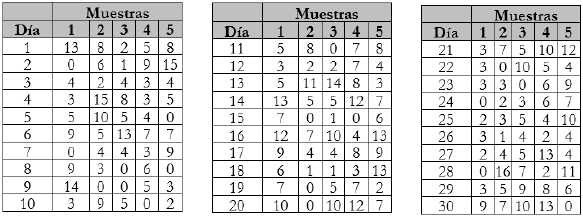
\includegraphics[scale=0.7]{FigurasUV/Datos.png}
  \caption{Datos del problema}
\end{figure}

\begin{itemize}
\item[a.] Construir un gr�fico de control X-barra; R con niveles de significancia del 5\% y del 0.27\%.

Los dos gr�ficos de control iniciales $\bar{x} - R$, para los niveles de significancia dados son:
\begin{figure}[h!]
  \centering
  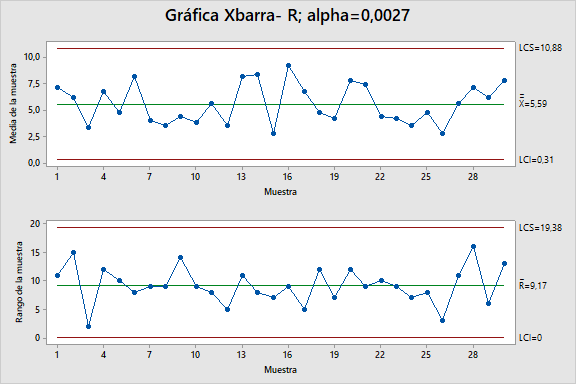
\includegraphics[scale=0.65]{FigurasUV/xbarra1.png}
  \caption{Gr�fico de control inicial $\bar{x} - R$ para $\alpha=0.0027$}
\end{figure}
\pagebreak
\begin{figure}[h!]
  \centering
  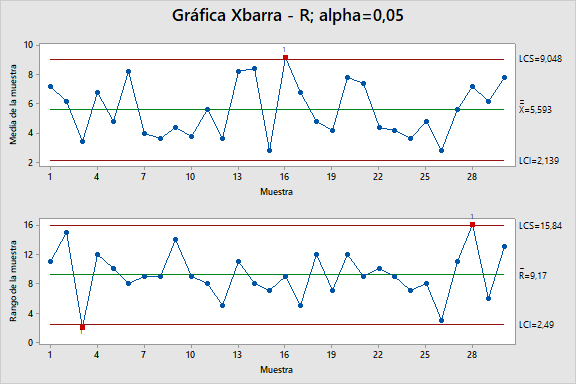
\includegraphics[scale=0.65]{FigurasUV/xbarra2.png}
  \caption{Gr�fico de control inicial $\bar{x} - R$ para $\alpha=0.05$}
\end{figure}

Podemos observar que en el gr�fico $\bar{x} - R$ para $\alpha=0.05$, tenemos tres puntos por fuera de los l�mites control, la muestra 16 en el de la media y las muestras 3 y 28 en el del rango, estos se deben eliminar para establecer el gr�fico. El gr�fico de control luego de eliminar estos dos puntos es:

\begin{figure}[h!]
  \centering
  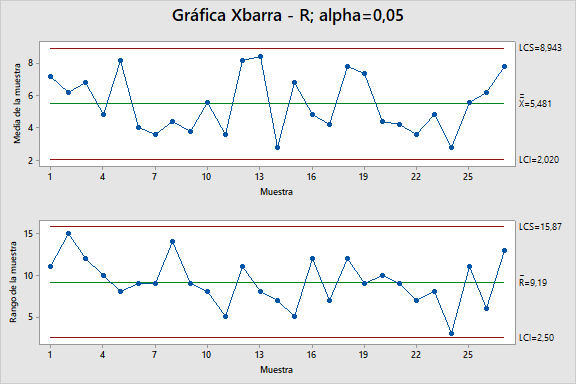
\includegraphics[scale=0.65]{FigurasUV/xbarra3.png}
  \caption{Gr�fico de control depurado $\bar{x} - R$ para $\alpha=0.05$}
\end{figure}

Se puede notar que el gr�fico con un nivel de significancia $\alpha=0.05$, genera limites m�s estrictos(estrechos) que su comparativo con $\alpha=0.0027$.

\item[b.] Simule 1000 subgrupos bajo control, desde la distribuci�n normal y evalu� la significancia de forma emp�rica para cada gr�fico.
\end{itemize}

\section{Punto 2}

Para controlar el volumen de llenado de un proceso de envasado se ha construido un gr�fico de control para el centramiento, obteniendo como resultado LSC= 1015; LIC= 995. Este gr�fico de control ha sido construido con un probabilidad de error tipo I equivalente a 0.6\%. Este proceso debe cumplir con un volumen de llenado nominal de 1000 cc con tolerancia de $\pm$ 30 ml. Haciendo uso de las observaciones con las que este gr�fico de control fue implementado, el controlador de calidad de dicho proceso ha realizado el correspondiente an�lisis de capacidad, reportando un �ndice Cpk=0,9348.

\begin{itemize}
\item[a.] Calcular los l�mites de control para el grafico S. (mantener el mismo nivel de error tipo I y el mismo tama�o de muestra)

\item[b.]

\item[c.]

\item[d.]

\end{itemize}





\section{Conclusi�n}




    \bibliography{references}


    \appendix% !don't modify this line�






\end{document}

